\chapter{Anonimato e Privacy}

Prima di analizzare le tecniche di anonimato all'interno della blockchain, è necessario definire con precisione cosa significhi questo termine in ambito informatico. Generalmente, il concetto si presta a due interpretazioni principali:
\begin{itemize}
    \item Interagire \textbf{senza utilizzare il proprio vero nome} (ma impiegando un alias testuale o numerico).
    \item Interagire \textbf{senza rivelare alcuna identità} o traccia riconducibile al singolo individuo.
\end{itemize}

Nel caso di Bitcoin, la prima interpretazione è chiaramente soddisfatta, poiché gli utenti utilizzano gli hash delle proprie chiavi pubbliche (gli indirizzi) come identità. Tuttavia, la seconda interpretazione non lo è. Questa distinzione ci porta a definire il sistema Bitcoin non come anonimo, bensì come \textbf{pseudo-anonimo}. 

Lo pseudo-anonimato, da solo, non è sufficiente a garantire la privacy su un registro pubblico. In crittografia, il vero anonimato si definisce come la somma di due proprietà: \textbf{Pseudo-anonimato + Unlinkability} (Non-collegabilità). 
L'\textit{unlinkability} è la proprietà per cui differenti interazioni dello stesso utente non possono essere correlate tra loro dal sistema o da un osservatore esterno. Per ottenere un'effettiva privacy in Bitcoin, dovrebbero verificarsi tre condizioni di \textit{unlinkability}:
\begin{itemize}
    \item Deve essere computazionalmente difficile ricollegare indirizzi diversi allo stesso utente reale.
    \item Deve essere difficile ricollegare transazioni diverse al medesimo utente.
    \item Deve essere difficile ricollegare il mittente di un pagamento al suo effettivo destinatario.
\end{itemize}

Mentre per i primi due casi è possibile adottare euristiche e buone pratiche (come generare un nuovo indirizzo per ogni transazione), il terzo caso è intrinsecamente violato dall'architettura base del protocollo: analizzando una singola transazione standard, il collegamento logico tra l'input (mittente) e l'output (destinatario) è pubblico e palese. Offuscare questo legame diventa fattibile solo se consideriamo la transazione non come un singolo evento isolato, ma come un flusso all'interno di un grafo di transazioni complesse.

Poiché garantire una completa \textit{unlinkability} sull'intero network è impossibile, l'obiettivo crittografico è quello di rendere anonima almeno una porzione delle transazioni, nascondendole all'interno di un \textbf{Anonymity Set} (Insieme di Anonimato). L'efficacia di queste tecniche dipenderà direttamente dal \textit{Threat Model}: dobbiamo cioè stabilire a priori \textbf{chi è l'attaccante e quali sono le sue capacità} di analisi della rete.

\section{Perché vogliamo l'anonimato?}
Poiché la blockchain è un \textit{ledger} (registro) completamente pubblico, l'assenza di anonimato comporta enormi criticità. Nel sistema bancario tradizionale, il registro delle transazioni è privato e custodito da un ente fiduciario; nessuno, tranne le autorità competenti, può accedere allo storico finanziario di un cittadino. Al contrario, in Bitcoin chiunque può ispezionare il registro, calcolare il saldo di una certa identità pseudo-anonima, e tracciarne ogni singolo movimento in entrata e in uscita.

Questa trasparenza estrema espone gli utenti a veri e propri tracciamenti finanziari. Se l'identità reale di un utente viene associata al suo indirizzo, è possibile per chiunque compiere azioni di spionaggio (ad esempio, un'azienda potrebbe monitorare i fornitori e i volumi d'affari di un competitor). 

Spesso si associa erroneamente la richiesta di anonimato finanziario ad attività illecite (acquisto di beni illegali, riciclaggio, evasione fiscale). Sebbene la tecnologia possa essere abusata, il diritto alla privacy finanziaria è un'esigenza legittima per proteggersi da sorveglianza di massa e attacchi mirati. Inoltre, anche i fondi di provenienza illecita, per poter essere utilizzati nell'economia reale, prima o poi devono transitare attraverso un punto di conversione in valuta \textit{fiat} (\textit{exchange} con procedure KYC/AML), rendendo di fatto possibile il tracciamento da parte delle forze dell'ordine. La neutralità della tecnologia crittografica è simile a quella della rete Tor: uno strumento \textit{agnostico} che fornisce privacy a prescindere dall'intento etico o meno dell'utente finale.

\subsection{Anonymous e-cash e Blind Signatures}
Una delle primissime e più eleganti soluzioni per i pagamenti digitali anonimi fu proposta dal crittografo David Chaum nel 1982. L'idea alla base di \textit{e-cash} era quella di consentire pagamenti digitali mantenendo una banca come autorità centrale fidata per la contabilità, ma impedendole matematicamente di tracciare le abitudini di spesa dei propri clienti.

Il protocollo si basa sul concetto crittografico delle \textbf{Blind Signatures} (Firme Cieche) e si articola in tre fasi:

\begin{itemize}
    \item \textbf{1. Fase di Prelievo (\textit{Withdrawal}):} L'utente Alice genera un numero seriale casuale $S$, che rappresenterà univocamente la moneta elettronica. Per nasconderlo alla banca, Alice applica una funzione di \textit{blinding} (mascheramento) utilizzando un fattore casuale $r$, ottenendo un \textit{commitment} $M = f(S, r)$. Alice invia $M$ alla banca richiedendo un prelievo.
    La banca autentica Alice, verifica i fondi sul suo conto e li detrae. Successivamente, la banca applica la propria firma digitale sul \textit{commitment} cieco, generando $\text{Sign}_{\text{bank}}(M)$, e la restituisce ad Alice. La banca ha firmato la moneta senza averne mai visto il vero numero seriale $S$.
    
    \item \textbf{2. Fase di Unblinding:} Ricevuta la firma cieca, Alice utilizza il fattore $r$ per rimuovere il mascheramento matematico applicato in precedenza. Grazie alle proprietà omomorfiche delle \textit{blind signatures}, questa operazione restituisce una firma della banca perfettamente valida applicata direttamente al seriale in chiaro: $\text{Sign}_{\text{bank}}(S)$.
    
    \item \textbf{3. Fase di Deposito (\textit{Deposit}):} Alice desidera acquistare un bene da Bob e gli consegna la moneta $(S, \text{Sign}_{\text{bank}}(S))$. Bob verifica crittograficamente la firma usando la chiave pubblica della banca e, per concludere la transazione, invia la moneta alla banca per farsi accreditare l'importo. La banca riceve il seriale $S$, verifica la propria firma e controlla nel suo database che $S$ non sia mai stato speso prima (prevenendo il \textit{Double Spending}). Se $S$ è nuovo, la banca accredita i fondi sul conto di Bob.
\end{itemize}

\textbf{La garanzia di Anonimato:} Durante il deposito, la banca vede il numero seriale $S$ per la prima volta. Non ha alcun modo crittografico per collegare questo seriale $S$ al \textit{commitment} $M$ che aveva firmato ad Alice durante la fase di prelievo. Di conseguenza, pur mantenendo il controllo assoluto contro la doppia spesa, l'autorità centrale non può assolutamente sapere chi ha pagato Bob, garantendo così un anonimato totale e matematicamente provato per il pagatore.

\begin{figure}[H]
    \centering
    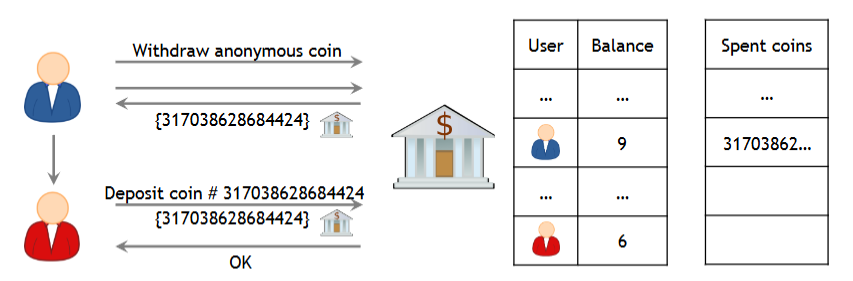
\includegraphics[width=0.9\linewidth]{Images/capitolo_4/transazione_blind.png}
\end{figure}
Naturalmente, per garantire tale anonimato abbiamo bisogno di spese unitarie o, al più, un numero limitato di quantità "prestabilite" in maniera tale che la banca non possa fare linking mediante la cifra spesa. Si presuppone chiaramente che il sistema sia utilizzato da più persone poiché altrimenti il link risulta banale.

Il vero e proprio problema è il fatto che i protocolli interattivi con la banca sono complicati da gestire e da decentralizzare soprattutto.

\subsection{Anonimato grazie a nuovi indirizzi}
Supponiamo che A voglia ottenere il massimo anonimato dal sistema blockchain e che, intuitivamente, decide di usare sempre indirizzi diversi per ogni transazione. 

Siamo adesso nella situazione in cui A voglia comprare un oggetto e, per farlo, necessita di un certo numero di monete che sono, quindi, dentro tanti UTXO diversi che hanno una firma diversa.
\begin{figure}[H]
    \centering
    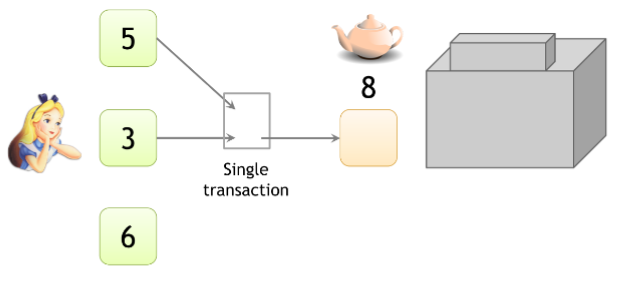
\includegraphics[width=0.6\linewidth]{Images/capitolo_4/tegliera.png}
\end{figure}
Poiché un attaccante vede una transazione verso una certa autorità, \footnote{Vedremo dopo come questa cosa venga capita} questo vede prima la transazione di compattazione degli uTXO e, quindi, riesce a collegare che quei due UTXO appartenevano alla stessa entità. Non solo, se il pagamento non è per intero, allora è necessario dare il resto che, quindi, apparterrà alla stessa entità del pagamento.

Tramite queste intuizioni, possiamo tracciare un grafo di questo tipo:
\begin{figure}[H]
    \centering
    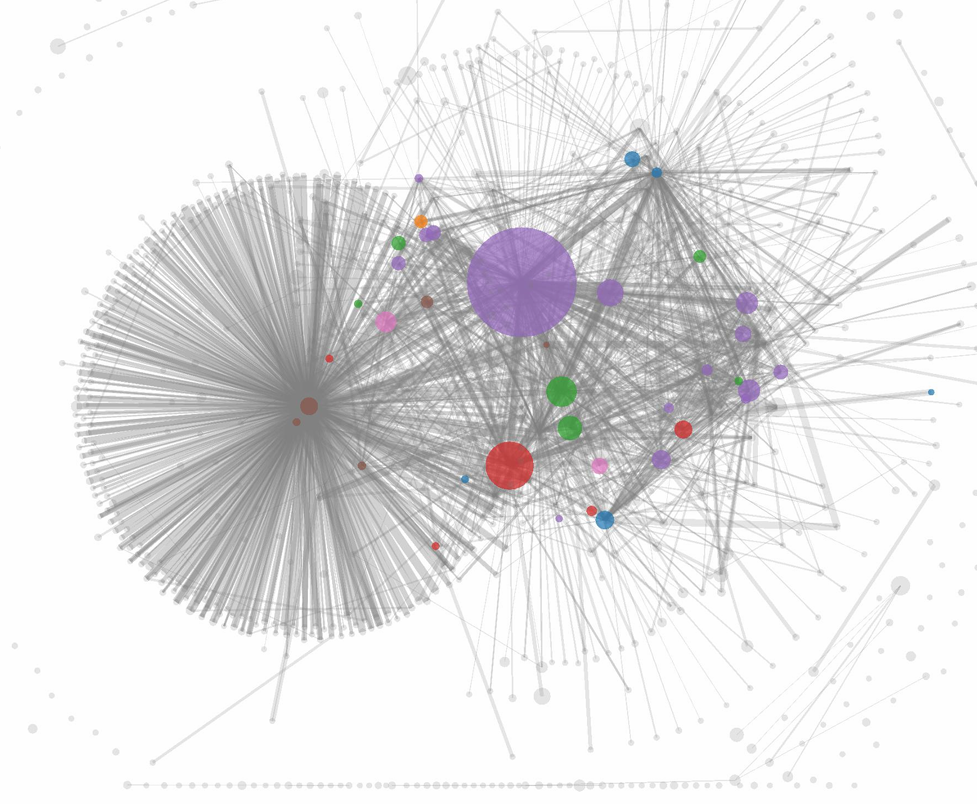
\includegraphics[width=0.6\linewidth]{Images/capitolo_4/grafo_conoscenza.png}
\end{figure}
Possiamo notare che quelli che ricevono tante transazioni sono, in genere, le autorità di cui parlavamo prima. Tra queste, possiamo trovare le più note \textbf{silkroad, satoshi dice, ecc.}.
Siamo a tutti gli effetti riusciti a capire come individuare le grossi autorità ma non è ancora ben chiaro come possiamo a tutti gli effetti deanonimizzare i singoli utenti. Per farlo, l'approccio più semplice è quello del \textit{social engineering}:
\begin{itemize}
    \item \textbf{Transazioni dirette:} Se io faccio in modo che qualcuno mi paghi, trovo il suo indirizzo e, tramite il blockchain explorer, posso vedere quanto si aveva nel portafoglio, da chi ha ricevuto questi soldi ecc.
    \item \textbf{Fornitori di Servizi:} Poiché non tutti possono minare Bitcoin, la maggior parte li compra da servizi esterni come binance e quei servizi devono per leggere conoscere l'identità della persona.
    \item \textbf{Careless:} La gente può deanonimizzarsi da sola pubblicando l'indirizzo online per ricevere donazioni ecc.
    \item \textbf{Attacchi retroattivi:} Poiché vengono scoperte algoritmi sempre più efficaci per raggruppare indirizzi e dato che la blockchain è immutabile, è possibile che in futuro venga scoperto un modo ancora più forte per deanonimizzare qualcuno.
\end{itemize}